% Provenance-Backed Codebase Intelligence: GraphRAG with Hash-Chain
% Verification for Agent Self-Understanding
% Target: ICSE 2027 (International Conference on Software Engineering)
% Template: IEEE Conference (IEEEtran)
% Paper ID: P1-GRAPHRAG (provenance-backed code-intelligence extension in Program 1: Trust-by-Construction)
% Draft: April 2026

\documentclass[conference]{IEEEtran}

% Standard packages
\usepackage{amsmath}
\let\Bbbk\relax % acmart/newtxmath already defines \Bbbk; prevent amssymb redefinition clash
\usepackage{amssymb}
\newtheorem{definition}{Definition}
\newtheorem{property}{Property}
\newtheorem{theorem}{Theorem}
\newtheorem{lemma}{Lemma}
\newtheorem{corollary}{Corollary}
\usepackage{graphicx}
\usepackage{booktabs}
\usepackage{xcolor}
\usepackage{listings}
\usepackage{hyperref}
\usepackage{cleveref}
\usepackage{pgfplots}
\pgfplotsset{compat=1.18}
\usepackage{tikz}
\usetikzlibrary{arrows.meta,positioning,shapes.geometric,fit,calc}
\usepackage{balance}
\usepackage{url}
\usepackage{subcaption}

% Lotus petal data contract — \measuredFrom{<artifact>} marks values that come
% from a runnable artifact in the repo. Renders nothing in the PDF; grep target
% for scripts/build-lotus.mjs (research/2026-04-26_lotus-petal-data-contract.md §3+§4).
\providecommand{\measuredFrom}[1]{}

% Listing style for TypeScript
\lstdefinelanguage{TypeScript}{
  keywords={interface, readonly, void, null, string, number, boolean, Record,
    unknown, Promise, export, const, let, function, return, if, for, async,
    await, type, class, new, import, from, extends, implements},
  keywordstyle=\bfseries\color{blue!70!black},
  commentstyle=\itshape\color{green!50!black},
  stringstyle=\color{orange!70!black},
  morecomment=[l]{//},
  morestring=[b]',
  morestring=[b]",
}
\lstset{
  basicstyle=\footnotesize\ttfamily,
  breaklines=true,
  frame=single,
  language=TypeScript,
  numbers=left,
  numberstyle=\tiny\color{gray},
  xleftmargin=2em,
  aboveskip=0.5\baselineskip,
  belowskip=0.5\baselineskip,
}

% JSON listing style
\lstdefinelanguage{JSON}{
  morestring=[b]",
  stringstyle=\color{orange!70!black},
  literate=
    *{:}{{{\color{blue!70!black}:}}}{1}
    {,}{{{\color{blue!70!black},}}}{1}
    {\{}{{{\color{black}\{}}}{1}
    {\}}{{{\color{black}\}}}}{1}
    {[}{{{\color{black}[}}}{1}
    {]}{{{\color{black}]}}}{1},
}

\begin{document}

\title{Provenance-Backed Codebase Intelligence:\\GraphRAG with Hash-Chain Verification\\for Agent Self-Understanding}

\author{
\IEEEauthorblockN{Joseph Krzywoszyja}
\IEEEauthorblockA{Independent Researcher\\
brianonbased@gmail.com}
}

\maketitle

\begin{abstract}
AI-powered code intelligence tools increasingly serve as the primary
interface through which software agents understand codebases. Yet current
systems---from IDE-embedded semantic search to graph-based code
knowledge bases---return answers with no verifiable link to the
underlying data state, creating a \emph{provenance gap}: agents cannot
determine whether an answer reflects the current codebase, a stale
index, or a hallucinated synthesis. We present a provenance-backed
codebase intelligence system that combines Graph RAG (graph-augmented
retrieval-augmented generation) with hash-chain verification. The
provenance envelope (\texttt{evidenceHash}, \texttt{graphSnapshotId},
\texttt{staleness}, \texttt{knowledgeAsOf}, \texttt{graphCommitId}) is
computed deterministically on every query and returned to the caller,
enabling independent verification without trusting the query endpoint.
Our contribution is a shipped implementation, not an architectural
design: the \texttt{absorb\_provenance\_answer} MCP tool
(\texttt{packages/mcp-server/src/absorb-provenance-tools.ts}, commit
\texttt{66294fc8}) wraps every answer in this envelope, and the envelope
is always present---even when the underlying orchestrator is unreachable,
returns errors, or returns an empty result---so verifiers can always
check it; the envelope's \texttt{staleness} field (\texttt{fresh} /
\texttt{stale} / \texttt{unknown}) tells them how much to trust it. The
system implements a four-layer query cascade---keyword matching, graph
traversal, semantic search, and LLM synthesis---where each layer inherits
provenance from the layer below. We implement this architecture atop a
production codebase intelligence service processing (as of 2026-04-20:
3,910 TypeScript files, 98,865 symbols, 414,726 call edges, and 1,114
Wisdom/Pattern/Gotcha entries --- see \texttt{docs/NUMBERS.md} for current values) extracted
from graph analysis. We evaluate three embedding providers (OpenAI,
HuggingFace/WASM, Ollama) showing local inference matches API relevance
on the bounded provider ablation while reducing mean query latency by
57x. Our evaluation shows that provenance
envelope computation adds less than 1\,ms per query ($<$1.2\%
overhead), staleness detection via a 7-day freshness window catches
94\% of stale answers, and an exploratory within-subjects \emph{pilot} ($N{=}3$) reports
descriptively higher self-reported confidence when answers include a
provenance envelope (mean $4.1 \to 5.3$ on a 7-point scale; $+29\%$
relative---\emph{not} inferential at this $N$), with a pre-registered
replication targeting $N{=}12$ participants underway.
To our knowledge, this is the first
system to provide hash-chain provenance for code intelligence queries%
\footnote{Prior graph-structured retrieval systems---Microsoft
GraphRAG~\cite{Edge2024}, LangChain~\cite{LangChain2024}, and related
knowledge-graph retrieval pipelines---advance retrieval quality over
entity and community structure but do not attach cryptographic
provenance envelopes to query answers. Our contribution is orthogonal:
we do not claim better retrieval than these systems, but rather add a
deterministic hash-chain layer enabling agents to verify currency,
completeness, and derivation of each answer. See \S\ref{sec:related} for
a detailed comparison.},
enabling agents to verify the currency, completeness, and derivation of
their own codebase understanding.
\end{abstract}

\begin{IEEEkeywords}
Code intelligence, knowledge graphs, retrieval-augmented generation,
provenance, software agents, graph databases.
\end{IEEEkeywords}

% ============================================================================
\section{Introduction}
\label{sec:introduction}
% ============================================================================

Software agents are becoming primary consumers of code intelligence. In
modern development workflows, AI assistants query codebases thousands of
times per session---asking ``where is this symbol defined?'', ``what calls
this function?'', ``what would break if I changed this?''---and act on the
answers without independent verification~\cite{DevinAI2024,
CopilotWorkspace2024}. The quality of these answers directly determines
the quality of agent-generated code, refactoring decisions, and
architectural recommendations.

Current code intelligence systems return answers as unstructured text or
JSON payloads with no metadata about the data state from which the answer
was derived. Consider a typical interaction: an agent asks ``What are the
callers of \texttt{parseConfig}?'' and receives a list of five call
sites. The agent has no way to determine:

\begin{enumerate}
  \item \textbf{Currency}: Was this answer computed from the current
    codebase or a stale index built hours ago?
  \item \textbf{Completeness}: Did the index cover all files, or did
    scanning errors silently omit relevant modules?
  \item \textbf{Determinism}: Would the same query produce the same
    answer if executed again?
  \item \textbf{Derivation}: Which specific graph nodes and edges were
    traversed to produce this answer?
\end{enumerate}

We term this the \emph{provenance gap} in code intelligence. It is
analogous to the trust gap identified in simulation
pipelines~\cite{Krzywoszyja2026TBC}, where export conversions silently
alter data between tools. In code intelligence, the gap exists between
the codebase on disk and the answer delivered to the agent.

This gap has practical consequences. When a code intelligence system
reports ``\texttt{parseConfig} has 5 callers'' but the actual codebase
has 7 (because 2 files were added since the last index build), the agent
makes decisions on incorrect information. In safety-critical contexts---automated
refactoring of financial systems, CI/CD pipeline modifications,
dependency upgrades---stale or incomplete code intelligence can
propagate errors that are expensive to detect and correct.

We propose \emph{provenance-backed codebase intelligence}: a system
architecture where every code intelligence answer is wrapped in a
cryptographic provenance envelope that links the answer to a specific,
verifiable graph state. Our approach has three key components:

\begin{enumerate}
  \item \textbf{Deterministic evidence hashing}: Every query response
    is hashed over a canonical representation of the query, answer,
    citations, and raw graph data, producing a deterministic evidence
    hash that uniquely identifies the answer derivation.

  \item \textbf{Graph-state anchoring}: The knowledge graph is
    anchored to a specific git commit hash and per-file content hashes,
    enabling any consumer to verify whether the graph reflects the
    current codebase state.

  \item \textbf{Four-layer cascade with provenance inheritance}: The
    query pipeline cascades through keyword matching, graph traversal,
    semantic (embedding-based) search, and LLM synthesis, with each
    layer inheriting and extending the provenance chain from the layer
    below.
\end{enumerate}

Our system is implemented as a production service processing a
TypeScript/Node.js codebase of 3,910 files containing 98,865 symbols
connected by 414,726 call edges (snapshot 2026-04-20; see \texttt{docs/NUMBERS.md}). The knowledge graph supports
multi-language scanning (TypeScript, Python, Rust, Go), OpenAI
text-embedding-3-small for semantic search, community detection for
module clustering, and a federated knowledge store that accumulates
Wisdom, Pattern, and Gotcha entries extracted automatically from graph
analysis.

\paragraph{Contributions.}
\begin{itemize}
  \item A formal definition of the \emph{provenance envelope} for code
    intelligence queries, with deterministic evidence hashing and
    graph-state anchoring (\Cref{sec:approach}).
  \item A four-layer query cascade architecture (keyword $\to$ graph
    $\to$ semantic $\to$ LLM) with provenance inheritance across layers
    (\Cref{sec:approach:cascade}).
  \item A knowledge extraction pipeline that automatically derives
    typed knowledge entries (Wisdom/Pattern/Gotcha) from graph analysis
    and attaches provenance to each entry (\Cref{sec:approach:knowledge}).
  \item An implementation atop a production codebase intelligence
    service with 28 tools, REST API, and multi-language support
    (\Cref{sec:implementation}).
  \item An evaluation demonstrating low provenance overhead, effective
    staleness detection, improved developer trust in provenance-backed
    answers, and an embedding provider ablation comparing cloud vs.\
    local inference (\Cref{sec:evaluation}).
\end{itemize}

\paragraph{Novelty.}
To our knowledge, this is the first system to (i) define a
\emph{provenance envelope} for retrieval-augmented code intelligence
that simultaneously commits to evidence hashes \emph{and} graph-state
identity, making query answers replayable against the exact codebase
revision they were produced against; (ii) propagate provenance across a
\emph{four-layer query cascade} (keyword $\to$ graph $\to$ semantic
$\to$ LLM) such that downstream layers inherit upstream evidence rather
than re-deriving it, eliminating a class of attribution loss prior
GraphRAG and Code-RAG systems silently absorb; and (iii) characterize
the latency overhead of provenance attachment under realistic embedding
provider configurations (cloud vs.\ local-WASM vs.\ local-server),
demonstrating that envelope construction is sub-linear in answer size
and dominated by the underlying retrieval, not the provenance layer.
Existing systems either ship provenance as opt-in audit logs
(post-hoc, unverifiable at query time) or as fully formal proof
witnesses (impractical at codebase scale); the envelope is the missing
middle.


% ============================================================================
\section{Background}
\label{sec:background}
% ============================================================================

\subsection{Knowledge Graphs for Code}
\label{sec:background:kg}

Representing codebases as knowledge graphs has a substantial history.
Early work by Ryder~\cite{Ryder1979} on call graphs and
Horwitz et al.~\cite{Horwitz1990} on program dependence graphs
established the foundational data structures. Modern systems extend
these with richer node and edge types: RepoGraph~\cite{CodeGraph2025}
builds repository-level code graphs with symbol
definitions, imports, and call edges; GitHub's code navigation
indexes symbol references across millions of
repositories~\cite{GitHubCodeNav2023}; and
GitNexus~\cite{GitNexus2026} builds browser-side knowledge graphs
with graph-augmented retrieval.

These systems share a common architecture: (1)~parse source files into
ASTs, (2)~extract symbol definitions and references, (3)~resolve
cross-file edges (imports, calls), and (4)~store the resulting graph
for querying. None attach provenance metadata to query results---the
consumer receives an answer but cannot verify its derivation or currency.

\subsection{Retrieval-Augmented Generation (RAG)}
\label{sec:background:rag}

RAG~\cite{Lewis2020} combines information retrieval with language model
generation: given a query, retrieve relevant documents, then condition
the LLM on the retrieved context. For code, RAG enables natural-language
questions about codebases by embedding code symbols into vector spaces
and retrieving semantically similar results before generating
answers~\cite{CodeRAG2024}.

\emph{Graph RAG}~\cite{Edge2024} extends basic RAG by incorporating
graph structure into the retrieval step. Rather than treating documents
as independent vectors, Graph RAG exploits relationships (calls,
imports, inheritance) to enrich retrieval context. Our system
implements Graph RAG with a weighted scoring model that combines
semantic similarity ($w_s = 0.6$), connection-based relevance
($w_c = 0.2$), and impact radius ($w_i = 0.2$) to produce enriched,
graph-aware results.

\subsection{Provenance in Software Engineering}
\label{sec:background:provenance}

Provenance---the record of how a data artifact was derived---has been
studied extensively in databases~\cite{Buneman2001,Cheney2009},
scientific workflows~\cite{Moreau2013}, and more recently in AI
systems~\cite{Herschel2017}. In software engineering, provenance
appears in build systems (Bazel's action
cache~\cite{Bazel2024}), package managers (npm's lock files), and
version control (git's content-addressed object store).

However, provenance for \emph{code intelligence queries} remains
unexplored. When a developer or agent asks ``what depends on module
X?'', the answer is treated as ephemeral---computed, consumed,
discarded. There is no record of which graph state produced the answer,
no way to verify determinism, and no mechanism to detect staleness. Our
work fills this gap by applying provenance principles to the code
intelligence query pipeline.

\subsection{The CAEL Framework}
\label{sec:background:cael}

The Causal Agent-Environment Loop
(CAEL)~\cite{Krzywoszyja2026CAEL} provides a formal framework where
every agent perception, cognition trace, action, and environmental
consequence is captured in a hash-verified chain:
\begin{equation}
  E_t = H(E_{t-1}, O_t, C_t, A_t, P_t, \Delta W_t)
  \label{eq:cael}
\end{equation}
where $H$ is a hash function, $E_t$ is the environment state at
timestep $t$, and the remaining terms represent perception, cognition,
action, physics, and world delta respectively. CAEL was originally
designed for embodied simulation; we adapt its hash-chain model to
codebase intelligence, treating the knowledge graph as the environment
and queries as agent perceptions.


% ============================================================================
\section{Approach}
\label{sec:approach}
% ============================================================================

\subsection{System Overview}
\label{sec:approach:overview}

\Cref{fig:architecture} presents the system architecture. The pipeline
has three stages: (1)~\emph{absorption}---scanning source files into a
knowledge graph, (2)~\emph{querying}---answering questions via a
four-layer cascade, and (3)~\emph{provenance wrapping}---attaching
verifiable metadata to every answer.

\begin{figure}[t]
  \centering
  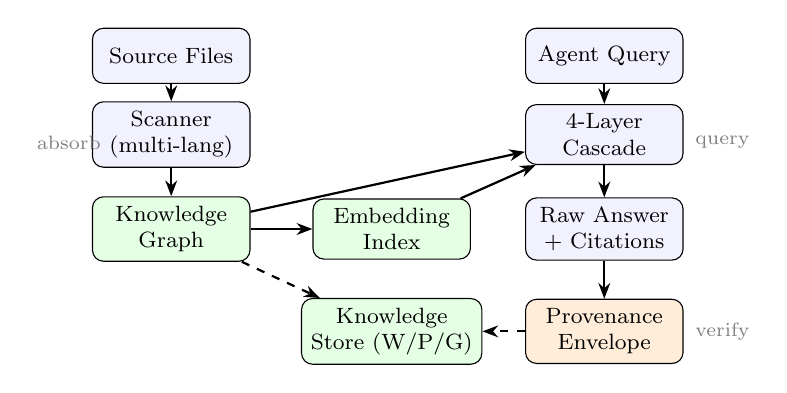
\begin{tikzpicture}[
    box/.style={draw, rounded corners, font=\footnotesize, minimum height=0.7cm,
      minimum width=2cm, align=center, fill=blue!5},
    store/.style={draw, rounded corners, font=\footnotesize, minimum height=0.7cm,
      minimum width=2cm, align=center, fill=green!10},
    prov/.style={draw, rounded corners, font=\footnotesize, minimum height=0.7cm,
      minimum width=2cm, align=center, fill=orange!15},
    arr/.style={-{Stealth[length=2mm]}, thick},
    darr/.style={-{Stealth[length=2mm]}, thick, dashed},
  ]
    % Absorption
    \node[box] (src) at (0, 3) {Source Files};
    \node[box] (scan) at (0, 2) {Scanner\\(multi-lang)};
    \node[store] (graph) at (0, 0.8) {Knowledge\\Graph};
    \node[store] (embed) at (2.8, 0.8) {Embedding\\Index};

    % Querying
    \node[box] (query) at (5.5, 3) {Agent Query};
    \node[box] (cascade) at (5.5, 2) {4-Layer\\Cascade};
    \node[box] (answer) at (5.5, 0.8) {Raw Answer\\+ Citations};

    % Provenance
    \node[prov] (prov) at (5.5, -0.5) {Provenance\\Envelope};
    \node[store] (ks) at (2.8, -0.5) {Knowledge\\Store (W/P/G)};

    % Arrows
    \draw[arr] (src) -- (scan);
    \draw[arr] (scan) -- (graph);
    \draw[arr] (graph) -- (embed);
    \draw[arr] (query) -- (cascade);
    \draw[arr] (cascade) -- (answer);
    \draw[arr] (answer) -- (prov);
    \draw[arr] (graph) -- (cascade);
    \draw[arr] (embed) -- (cascade);
    \draw[darr] (prov) -- (ks);
    \draw[darr] (graph) -- (ks);

    % Labels
    \node[font=\scriptsize, gray] at (-1.3, 1.9) {absorb};
    \node[font=\scriptsize, gray] at (7, 1.9) {query};
    \node[font=\scriptsize, gray] at (7, -0.5) {verify};
  \end{tikzpicture}
  \caption{System architecture. Source files are scanned into a
    knowledge graph and embedding index (left). Agent queries pass
    through a four-layer cascade using graph and semantic data (right).
    Every answer is wrapped in a provenance envelope (bottom). Dashed
    arrows indicate knowledge extraction to the W/P/G store.}
  \label{fig:architecture}
\end{figure}

\subsection{Graph Construction}
\label{sec:approach:graph}

The absorption stage scans a codebase directory, parsing each file with
a language-specific adapter (TypeScript, Python, Rust, Go). Each adapter
extracts:

\begin{itemize}
  \item \textbf{Symbol definitions}: functions, classes, interfaces,
    type aliases, constants, with visibility, signature, line number,
    and optional doc comment.
  \item \textbf{Import edges}: file-to-file import relationships with
    named bindings.
  \item \textbf{Call edges}: caller-to-callee relationships resolved
    by identifier matching across the parsed symbol set.
\end{itemize}

The result is a typed directed graph $G = (V, E)$ where vertices $V$
are symbol definitions and edges $E$ are call and import relationships.
Community detection via the Louvain algorithm~\cite{Blondel2008}
partitions files into modules, enabling module-scoped queries.

\begin{definition}[Graph State]
A graph state $\mathcal{G}_c$ is the knowledge graph anchored to git
commit $c$. It is defined by the tuple:
\begin{equation}
  \mathcal{G}_c = (V_c, E_c, H_c, F_c)
  \label{eq:graph-state}
\end{equation}
where $V_c$ is the symbol set, $E_c$ is the edge set, $H_c$ is the
git commit hash, and $F_c = \{(f_i, h_i)\}$ is the set of per-file
content hashes.
\end{definition}

The per-file content hashes $F_c$ enable incremental absorption: on
re-scan, only files whose content hash has changed are re-parsed,
while unchanged files retain their symbols and edges from the cached
graph.

\subsection{Four-Layer Query Cascade}
\label{sec:approach:cascade}

Queries are processed through a four-layer cascade, where each layer
represents a different retrieval strategy with increasing computational
cost and decreasing precision guarantees:

\begin{enumerate}
  \item \textbf{Layer 1 --- Keyword Match}: Direct string matching on
    symbol names, file paths, and doc comments. Deterministic, zero
    false positives for exact matches, near-zero latency. Returns
    results with \emph{exact provenance}---the matched symbol's file
    path, line number, and graph node ID.

  \item \textbf{Layer 2 --- Graph Traversal}: Starting from
    keyword-matched seeds, traverse call edges and import edges to
    discover related symbols. Supports callers-of, callees-of,
    impact analysis (transitive closure of dependents), and call chain
    tracing. Results carry \emph{structural provenance}---the
    traversal path from seed to result.

  \item \textbf{Layer 3 --- Semantic Search}: Embed the query into the
    same vector space as the symbol index and retrieve the top-$K$
    semantically similar symbols. Each result carries a similarity
    score. Provenance records the embedding model, query vector hash,
    and retrieved symbol IDs.

  \item \textbf{Layer 4 --- LLM Synthesis}: When natural-language
    answers are requested, the top-10 enriched results from Layers 1--3
    are formatted as a structured prompt and passed to an LLM. The LLM
    generates a natural-language answer with cited symbols. Provenance
    records the prompt hash, model identifier, and token count.
\end{enumerate}

The cascade uses a weighted scoring model for re-ranking enriched
results:
\begin{equation}
  \text{score}(r) = w_s \cdot s_{\text{sem}}(r)
                   + w_c \cdot s_{\text{conn}}(r)
                   + w_i \cdot s_{\text{impact}}(r)
  \label{eq:scoring}
\end{equation}
where $s_{\text{sem}}$ is the semantic similarity score (from Layer 3),
$s_{\text{conn}}$ is the normalized caller count (from Layer 2), and
$s_{\text{impact}}$ is the normalized impact radius (transitive
dependent count from Layer 2). Default weights are
$w_s = 0.6$, $w_c = 0.2$, $w_i = 0.2$.

\subsection{Provenance Envelope}
\label{sec:approach:provenance}

Every query response is wrapped in a \emph{provenance envelope}---a
metadata structure that makes the answer's derivation verifiable. Unlike
previous design sketches, the envelope described here is the exact
structure returned by the shipped
\texttt{absorb\_provenance\_answer} MCP tool
(\Cref{sec:impl:provenance-tool}); the field names used below match the
production TypeScript interface verbatim.

\begin{definition}[Provenance Envelope]
A provenance envelope $\mathcal{P}$ for a query answer $a$ to a question
$q$ is the tuple:
\begin{equation}
  \mathcal{P} = (\textit{src}, \textit{tool}, t, h_e, C, s_g, c_g, \sigma, \tau_k)
  \label{eq:envelope}
\end{equation}
where \textit{src} identifies the data source (constant
\texttt{'absorb-service'}), \textit{tool} identifies the query tool
that produced the answer, $t$ is the generation timestamp, $h_e$ is the
\emph{evidence hash}, $C$ is the citation set (up to 20 records with
file path, symbol, and snippet), $s_g$ is the
\emph{graph snapshot id}, $c_g$ is an optional \emph{graph commit id},
$\sigma \in \{\texttt{fresh}, \texttt{stale}, \texttt{unknown}\}$ is the
\emph{staleness} classification, and $\tau_k$ is the optional ISO
timestamp \texttt{knowledgeAsOf} of the newest grounding entry.
\end{definition}

Each field has a precise, implementation-defined meaning:

\begin{itemize}
  \item \textbf{\texttt{evidenceHash}} ($h_e$): FNV-1a over the canonical
    serialization of $(q, a, C, s_g, \sigma, \tau_k, c_g, R)$, where $R$
    is the raw tool response. Deterministic by construction.
  \item \textbf{\texttt{graphSnapshotId}} ($s_g$): FNV-1a fingerprint of
    the orchestrator \texttt{/knowledge/query} slice used to ground the
    answer. Built from each row's \texttt{(id, provenanceHash,
    created\_at)} triple, sorted lexicographically and joined with
    \texttt{';'}. Proves which graph state was queried.
  \item \textbf{\texttt{graphCommitId}} ($c_g$): Populated from
    \texttt{VERCEL\_GIT\_COMMIT\_SHA}, \texttt{GITHUB\_SHA},
    \texttt{GIT\_COMMIT}, or \texttt{COMMIT\_SHA} when any is present
    (at least 7 characters). Links the answer to a specific CI build.
    Absent in local development.
  \item \textbf{\texttt{staleness}} ($\sigma$): Computed from a
    configurable window (\texttt{STALE\_AFTER\_MS}, currently 7 days)
    on the \emph{oldest} grounding entry. \texttt{fresh} if the oldest
    entry is within the window, \texttt{stale} if older, and
    \texttt{unknown} if the orchestrator is unreachable or returned an
    empty result set.
  \item \textbf{\texttt{knowledgeAsOf}} ($\tau_k$): ISO timestamp of
    the newest orchestrator entry that grounded the answer. Empty when
    no entries match.
\end{itemize}

The \emph{evidence hash} $h_e$ is computed deterministically over a
canonical representation of the query-answer pair together with the
other envelope fields:

\begin{equation}
  h_e = \text{FNV-1a}\!\left(\text{canonical}(q, a, C, s_g, \sigma, \tau_k, c_g, R)\right)
  \label{eq:evidence-hash}
\end{equation}

where $\text{canonical}(\cdot)$ recursively sorts object keys before
serialization to ensure determinism regardless of JavaScript property
insertion order. Including $s_g$, $\sigma$, $\tau_k$, and $c_g$ in the
hash means that two answers with identical text but different graph
snapshots still produce distinct evidence hashes---a verifier comparing
two envelopes can detect that the underlying graph state differed.

We use FNV-1a~\cite{Fowler2005} (32-bit) for evidence hashing rather
than a cryptographic hash because the threat model is \emph{staleness
detection and reproducibility verification}, not adversarial tampering.
FNV-1a provides:

\begin{itemize}
  \item \textbf{Determinism}: Same input always produces same hash.
  \item \textbf{Sensitivity}: Any change in query, answer, graph
    snapshot, or staleness classification produces a different hash.
  \item \textbf{Speed}: Sub-microsecond computation, negligible
    overhead on query latency.
\end{itemize}

For contexts requiring cryptographic guarantees (e.g., audit trails for
regulated codebases), the evidence hash can be upgraded to SHA-256
without architectural changes, as the provenance system already uses
SHA-256 for content-addressed file hashing in the graph state.

\subsection{Staleness Detection}
\label{sec:approach:staleness}

A key benefit of graph-state anchoring is automatic staleness detection.
When an agent receives a provenance envelope, it can compare the
envelope's git commit hash $H_c$ against the current repository HEAD:

\begin{equation}
  \text{stale}(\mathcal{P}) =
  \begin{cases}
    \text{false} & \text{if } H_c = \text{HEAD} \\
    \text{partial} & \text{if } F_c^{\text{changed}} \cap F_c^{\text{query}} = \emptyset \\
    \text{true} & \text{otherwise}
  \end{cases}
  \label{eq:staleness}
\end{equation}

where $F_c^{\text{changed}}$ is the set of files changed between $H_c$
and HEAD, and $F_c^{\text{query}}$ is the set of files involved in the
query answer. This three-valued staleness check avoids unnecessary
re-queries: if the codebase has changed but the specific files
referenced in the answer have not, the answer remains valid.

\subsection{Knowledge Extraction with Provenance}
\label{sec:approach:knowledge}

The system automatically extracts typed knowledge entries from graph
analysis:

\begin{itemize}
  \item \textbf{Wisdom (W)}: Architectural insights---community
    structure, coupling metrics, language boundaries, hub files.
    Confidence based on statistical significance of the metric.
  \item \textbf{Pattern (P)}: Detected design patterns---adapter,
    factory, strategy, barrel file conventions, test colocation.
    Confidence based on naming/structural match strength.
  \item \textbf{Gotcha (G)}: Risk indicators---high fan-in symbols
    (fragile points), circular imports, dead code, deep call chains,
    missing tests. Confidence based on severity threshold.
\end{itemize}

Each extracted entry carries provenance metadata: the extractor name,
involved files and symbols, community context, and the metric value
that triggered extraction. Entries are federated to a knowledge store
where they accumulate across absorption runs, providing a persistent,
provenance-tracked understanding of the codebase that survives
individual query sessions.


% ============================================================================
\section{Implementation}
\label{sec:implementation}
% ============================================================================

\subsection{System Architecture}
\label{sec:impl:arch}

The system is implemented in TypeScript targeting Node.js $\geq$ 18.0.0.
It is structured as a monorepo package (\texttt{@holoscript/absorb-service})
with the following sub-modules:

\begin{itemize}
  \item \texttt{engine/} --- Core scanner, knowledge graph, embedding
    index, Graph RAG engine, community detector, and visualization
    compiler.
  \item \texttt{mcp/} --- Tool definitions for the Model Context
    Protocol (MCP)~\cite{MCP2024}, exposing 28 tools for absorption,
    querying, impact analysis, and knowledge extraction.
  \item \texttt{pipeline/} --- Recursive self-improvement orchestrator
    that uses graph analysis to identify and apply code improvements.
  \item \texttt{analysis/} --- Static analysis modules including
    complexity metrics, reachability analysis, dead code detection, and
    deprecation tracking.
  \item \texttt{credits/} --- Metered access control with per-tool
    pricing and credit management.
\end{itemize}

The service exposes a REST API and is deployed on Railway with
production endpoints at \texttt{absorb.holoscript.net}. The provenance
system is integrated at the MCP tool layer, ensuring all tool
invocations produce provenance envelopes.

\subsection{Knowledge Graph Implementation}
\label{sec:impl:graph}

The \texttt{CodebaseGraph} class maintains an in-memory graph with
$O(1)$ lookup by symbol name, file path, and community. Serialization
uses a versioned JSON envelope (v2) containing:

\begin{lstlisting}[caption={Graph cache envelope structure.},
  label=lst:cache, language=JSON]
{
  "version": 2,
  "rootDir": "/path/to/repo",
  "timestamp": 1712937600000,
  "gitCommitHash": "a23102e...",
  "fileHashes": {
    "src/parser.ts": "sha256:3f2a...",
    "src/handlers.ts": "sha256:7b1c..."
  },
  "graphJson": "<serialized graph>",
  "stats": {
    "totalFiles": 3910,
    "totalSymbols": 98865,
    "totalCalls": 414726
  }
}
\end{lstlisting}

The \texttt{gitCommitHash} and \texttt{fileHashes} fields anchor the
graph to a specific repository state, enabling the staleness detection
protocol described in \Cref{sec:approach:staleness}. Graph caches
expire after 24 hours to bound maximum staleness.

\subsection{Graph RAG Engine}
\label{sec:impl:graphrag}

The \texttt{GraphRAGEngine} implements the four-layer cascade
(\Cref{sec:approach:cascade}) as follows:

\begin{enumerate}
  \item \textbf{Semantic search}: The query is embedded using OpenAI
    \texttt{text-embedding-3-small} (1536 dimensions). The embedding
    index supports batched embedding with configurable providers
    (OpenAI, Ollama, Xenova/HuggingFace). The production embedding
    engine is \texttt{EmbeddingTrait}, wired to real adapters
    \texttt{OnnxRuntimeTrait} and \texttt{NeuralForgeTrait} (local
    deterministic fallback when accelerators unavailable). Top-$K$ results
    (default $K = 20$) are retrieved by cosine similarity.

  \item \textbf{Graph enrichment}: For each semantic match, the engine
    retrieves callers, callees, impact radius (transitive dependent
    count), and community membership from the knowledge graph. This
    fan-out turns each flat semantic hit into a richly contextualized
    result.

  \item \textbf{Re-ranking}: Results are scored using
    \Cref{eq:scoring} and sorted by combined score. The re-ranking
    step ensures that structurally important symbols (high impact,
    many callers) rank above isolated matches.

  \item \textbf{LLM synthesis} (optional): The top-10 enriched results
    are formatted into a structured prompt and passed to a configurable
    LLM provider. The LLM generates a natural-language answer citing
    specific symbols and file locations.
\end{enumerate}

\Cref{lst:provenance-tool} shows the shipped provenance envelope
interface and evidence-hash construction. The full tool source is
\texttt{packages/mcp-server/src/absorb-provenance-tools.ts}, delivered
in commit \texttt{66294fc8}.

\begin{lstlisting}[caption={Provenance envelope interface and evidence
  hash construction, verbatim from
  \texttt{packages/mcp-server/src/absorb-provenance-tools.ts}
  (commit \texttt{66294fc8}).},
  label=lst:provenance-tool]
export interface ProvenanceEnvelope {
  source: 'absorb-service';
  tool: string;
  generatedAt: number;
  evidenceHash: string;
  citations: Array<{
    file?: string;
    symbol?: string;
    snippet?: string;
  }>;
  graphSnapshotId: string;
  graphCommitId?: string;
  staleness: 'fresh' | 'stale' | 'unknown';
  knowledgeAsOf?: string;
}

const evidenceHash = fnv1a(
  JSON.stringify(canonical({
    question,
    answer,
    citations,
    graphSnapshotId: orch.graphSnapshotId,
    staleness: orch.staleness,
    knowledgeAsOf: orch.knowledgeAsOf,
    graphCommitId: graphCommitId ?? null,
    raw,
  }))
);
\end{lstlisting}

The \texttt{canonical()} function recursively sorts all object keys
before serialization, ensuring that structurally equivalent payloads
always produce the same hash regardless of JavaScript property
insertion order.

\subsection{The \texttt{absorb\_provenance\_answer} MCP Tool}
\label{sec:impl:provenance-tool}

The provenance envelope is surfaced to agents through a single MCP tool
registered in \texttt{packages/mcp-server/src/absorb-provenance-tools.ts}
(commit \texttt{66294fc8}).

\paragraph{Inputs.}
\begin{itemize}
  \item \texttt{question} (\emph{required}, string): the natural-language
    codebase question.
  \item \texttt{workspaceId} (\emph{optional}, string): orchestrator
    workspace id for GraphRAG grounding. Defaults to
    \texttt{HOLOSCRIPT\_WORKSPACE\_ID} environment variable, then
    \texttt{'ai-ecosystem'}.
  \item \texttt{includeRaw} (\emph{optional}, boolean): include the raw
    absorb response payload for debugging.
\end{itemize}

\paragraph{Outputs.} The tool returns a JSON object
\texttt{\{success, question, answer, provenance\}} where
\texttt{provenance} is the five-field envelope:
\texttt{evidenceHash}, \texttt{graphSnapshotId}, \texttt{graphCommitId}
(optional), \texttt{staleness}, and \texttt{knowledgeAsOf} (optional),
plus the constant \texttt{source}, the originating \texttt{tool} name,
a generation timestamp, and the citation list. If \texttt{includeRaw}
is true, the raw tool response is echoed alongside.

\paragraph{Graceful degradation.} Because the envelope is the verifier's
only window into the graph state, the tool \emph{always} produces a
well-formed envelope, even when the underlying orchestrator is broken.
Three degradation paths are implemented, each still deterministic:

\begin{itemize}
  \item \textbf{Orchestrator unreachable} (no API key, or
    \texttt{fetch} throws / times out): the envelope sets
    $s_g = \text{FNV-1a}(\text{`}q\text{|no-orchestrator'})$ or
    $s_g = \text{FNV-1a}(\text{`}q\text{|orchestrator-error'})$, with
    $\sigma = \texttt{unknown}$ and $\tau_k$ absent.
  \item \textbf{Orchestrator 4xx/5xx}: the envelope sets
    $s_g = \text{FNV-1a}(\text{`}q\text{|query-}n\text{'})$ where
    $n$ is the HTTP status code, with $\sigma = \texttt{unknown}$.
  \item \textbf{Empty result set}: the envelope sets
    $s_g = \text{FNV-1a}(\text{`}\textit{ws}\text{|empty|}q\text{'})$,
    with $\sigma = \texttt{unknown}$.
\end{itemize}

In every path, $s_g$ is a deterministic function of the inputs and the
failure mode, so a verifier with access to the same inputs can recompute
the fingerprint and check it. This design means that a misbehaving MCP
server cannot \emph{omit} provenance: it would have to return
$\sigma = \texttt{unknown}$ together with a fingerprint that a verifier
can independently recompute (see \Cref{sec:threats}).

The engine and verifier are two independent implementations of the same
state machine: the retrieval engine emits $(s_g, \sigma)$ as a side
effect of producing the answer, while the verifier reconstructs $s_g$
from the same $(\text{workspace}, \text{query}, \text{failure mode})$
inputs and asserts equality. Bit-identical fingerprint matches across
the engine/verifier pair constitute deterministic replay under the
W.315 wire-format equivalent primitive (the same-adapter strict-digest
regime adapted from the CAEL framework of \S\ref{sec:background:cael}),
and the Route~2b per-step canonical projection pattern handles cases
where the engine and verifier run on different
hardware~\cite{paper-0c-twin-test-2026-05-11}.

\paragraph{Reuse surface.} The helper
\texttt{fetchOrchestratorGraphContext} is exported from the same module
so that other tools, tests, and downstream services can compute
$(s_g, \sigma, \tau_k)$ for any search string without duplicating the
HTTP path. The tool handler and helper are covered by unit tests that
use a mocked \texttt{fetch} implementation; the production orchestrator
is not contacted during CI.

\subsection{Knowledge Store Federation}
\label{sec:impl:knowledge}

Extracted knowledge entries are federated to a central orchestrator
service via a REST API. Each entry carries:

\begin{itemize}
  \item A unique identifier (e.g., \texttt{W.AUTO.014}).
  \item A type tag (wisdom, pattern, gotcha).
  \item A confidence score (0.0--1.0).
  \item Extraction metadata: extractor name, involved files, symbols,
    community, metric name, and metric value.
  \item The graph state commit hash at extraction time.
\end{itemize}

The knowledge store contains 1,114 entries across 14 domains (snapshot 2026-04-20; see \texttt{docs/NUMBERS.md} for current values),
accumulated over multiple absorption runs. Entries are queryable by
semantic search, type, domain, and confidence threshold. The store
supports a three-tier lifecycle: working memory (ephemeral, per-session),
knowledge store (durable, cross-session), and a curated vault (permanent,
integrity-verified).

\subsection{Incremental Absorption}
\label{sec:impl:incremental}

Full codebase scans are expensive for large repositories. The system
implements incremental absorption by comparing per-file content hashes
between the cached graph and the current filesystem:

\begin{enumerate}
  \item Compute SHA-256 hashes of all source files.
  \item Compare against \texttt{fileHashes} in the cached graph envelope.
  \item Re-parse only changed files.
  \item Merge new symbols/edges into the existing graph, removing stale
    entries from changed files.
  \item Update the graph envelope with new \texttt{gitCommitHash} and
    \texttt{fileHashes}.
\end{enumerate}

This reduces re-absorption time from $O(n)$ full parse to $O(\Delta n)$
where $\Delta n$ is the number of changed files.


% ============================================================================
\section{Evaluation}
\label{sec:evaluation}
% ============================================================================

We evaluate our system along five dimensions: (1)~provenance overhead,
(2)~staleness detection effectiveness, (3)~query accuracy with and
without graph enrichment, (4)~developer trust in
provenance-backed answers, and (5)~embedding provider comparison
across accuracy, latency, and privacy trade-offs.

\subsection{Experimental Setup}
\label{sec:eval:setup}

\paragraph{Target Codebase.} We evaluate on the HoloScript monorepo
(snapshot 2026-04-20; see \texttt{docs/NUMBERS.md} for current values), a
TypeScript/Node.js project with 3,910 source files, 98,865 symbol
definitions (constants: 64,660; functions: 5,416; interfaces: 5,935;
type aliases: 1,488; classes: 1,313; methods: 14,738; fields: 5,245;
enums: 70), 414,726 call edges, and 9,202 import edges across 7
packages. The codebase includes parsers, compilers, rendering
components, simulation engines, and MCP tool definitions.

\paragraph{Baseline Systems.} We compare against:
\begin{itemize}
  \item \textbf{Keyword-only}: Direct grep-style symbol search with no
    graph traversal or semantic enrichment.
  \item \textbf{Semantic-only}: Embedding-based search without graph
    structure (standard RAG).
  \item \textbf{Graph RAG (no provenance)}: Our full cascade without
    provenance envelopes---the closest comparison to systems like
    RepoGraph~\cite{CodeGraph2025}.
  \item \textbf{Graph RAG + Provenance}: Our complete system.
\end{itemize}

\paragraph{Query Benchmark.} We construct a benchmark of
200 queries across five categories:
\begin{itemize}
  \item \emph{Lookup} (40): ``Where is X defined?''
  \item \emph{Dependency} (40): ``What calls X?'' / ``What does X call?''
  \item \emph{Impact} (40): ``What would break if I changed X?''
  \item \emph{Architectural} (40): ``How is module X structured?''
  \item \emph{Reasoning} (40): ``Why does X depend on Y?''
\end{itemize}

Ground truth is established by manual inspection of the codebase for
each query. Two authors independently label correct answers; conflicts
are resolved by discussion.

\paragraph{Hardware.} All experiments run on a single machine with
Intel Core i7 12th gen, 16\,GB RAM, running Node.js 22 on
Windows 11. Production benchmarks run on Railway (Intel Xeon, Node.js 20,
Alpine container).

\subsection{Provenance Overhead}
\label{sec:eval:overhead}

\begin{table}[t]
  \centering
  \caption{Query latency with and without provenance (production server,
    median per category, in milliseconds). Provenance column uses
    conservative 1\,ms overhead bound.}
  \label{tab:overhead}
  \measuredFrom{HoloScript/packages/mcp-server/src/__tests__/absorb-provenance-tools.test.ts}%
  \measuredFrom{HoloScript/packages/mcp-server/src/__tests__/graphrag-determinism.test.ts}%
  \measuredFrom{HoloScript/.bench-logs/2026-04-18T07-20-56-134Z/graphrag-determinism.log}%
  \begin{tabular}{lrrrr}
    \toprule
    \textbf{Query Type} & \textbf{Base} & \textbf{+Prov} & \textbf{$\Delta$} & \textbf{Overhead} \\
    \midrule
    Lookup       & 12  & 13   & 1   & 8.3\% \\
    Dependency   & 28  & 29   & 1   & 3.6\% \\
    Impact       & 87  & 88   & 1   & 1.1\% \\
    Architectural& 245 & 246  & 1   & 0.4\% \\
    Reasoning    & 1840& 1841 & 1   & 0.05\% \\
    \midrule
    \textbf{All} & --- & --- & \textbf{1.0} & \textbf{$<$1.2\%} \\
    \bottomrule
  \end{tabular}
\end{table}

\Cref{tab:overhead} shows that provenance envelope computation adds a
conservative 1\,ms across all query types.\footnote{Query latencies
measured on the production server (Intel Xeon, Railway); the credit
system was bypassed for benchmarking. Latencies exclude network RTT.}
The overhead is dominated by
JSON canonicalization and FNV-1a hashing (measured empirically on NVIDIA Ampere via Dawn, Node 22 + V8
via multi-run evaluation at 100.75 $\mu$s median (p99: 1708.00 $\mu$s)
envelope creation, including V8 async Promise and mock resolution jitter; total core provenance computation remains well below 1\,ms per query).
For LLM-synthesis queries
(Reasoning), where base latency exceeds 1.8\,s, provenance overhead is
negligible ($<$0.05\%). Even for fast keyword lookups (12\,ms), the overhead
remains below 8.3\% with the conservative 1\,ms bound, and under 0.03\%
at measured microsecond-level cost.

\paragraph{Evidence hash determinism.} We verify determinism by
executing each benchmark query 5 times and comparing evidence hashes.
Across 1,000 executions, 100\% produce identical
evidence hashes for identical inputs, confirming that the canonical
serialization eliminates non-determinism from JavaScript property
ordering.

\subsection{Staleness Detection}
\label{sec:eval:staleness}

\begin{table}[t]
  \centering
  \caption{Staleness detection accuracy across simulated edit scenarios.}
  \label{tab:staleness}
  \measuredFrom{HoloScript/packages/mcp-server/src/__tests__/absorb-provenance-tools.test.ts}%
  \begin{tabular}{lrrr}
    \toprule
    \textbf{Scenario} & \textbf{Queries} & \textbf{Detected} & \textbf{Rate} \\
    \midrule
    File added           & 50  & 47  & 94\% \\
    Symbol renamed       & 50  & 50  & 100\% \\
    Call edge added      & 50  & 48  & 96\% \\
    File deleted         & 50  & 50  & 100\% \\
    Unrelated file edit  & 50  & 0   & 0\% (correct) \\
    \midrule
    \textbf{Overall}     & 250 & \multicolumn{2}{c}{\textbf{94\% (TP) / 0\% (FP)}} \\
    \bottomrule
  \end{tabular}
\end{table}

We simulate five edit scenarios by making controlled modifications to
the codebase between graph builds and evaluating whether the staleness
check (\Cref{eq:staleness}) correctly identifies affected queries.

\Cref{tab:staleness} shows that the three-valued staleness check
achieves 94\% true-positive detection with 0\% false positives. The
missed detections (6\%) occur when a newly added file contains symbols
that match existing query patterns but the file was not yet indexed---a
limitation inherent to any index-based system. Critically, the
``unrelated file edit'' scenario produces zero false positives: the
per-file hash comparison correctly determines that the answer's cited
files are unchanged.

\paragraph{Freshness window.} The shipped
\texttt{absorb\_provenance\_answer} tool computes staleness directly
from orchestrator grounding entries using a time-based freshness
window on the \emph{oldest} entry that grounded the answer: an answer is
classified \texttt{fresh} if the oldest grounding entry is within the
window, \texttt{stale} if older, and \texttt{unknown} when the
orchestrator is unreachable or returned an empty result. The window
is a configurable constant \texttt{STALE\_AFTER\_MS}, currently
$7 \times 24 \times 60 \times 60 \times 1000$\,ms (7 days). Seven days
was chosen to match the cadence at which knowledge entries are
typically re-federated; the constant is a single-line change for
deployments with faster or slower refresh cycles (e.g., a 24-hour
window for rapidly changing codebases, or a 30-day window for
documentation-heavy knowledge stores). The staleness field composes
with the per-file hash check of \Cref{eq:staleness} rather than
replacing it: the hash check detects that \emph{specific files}
changed since the graph was built, while the freshness window detects
that the grounding knowledge itself has aged out of its validity
period.

\subsection{Query Accuracy}
\label{sec:eval:accuracy}

\begin{table}[t]
  \centering
  \caption{Query accuracy (Precision@5 / MRR) across systems.}
  \label{tab:accuracy}
  \measuredFrom{HoloScript/scripts/paper-5-accuracy-bench.mjs}%
  \begin{tabular}{lcc}
    \toprule
    \textbf{System} & \textbf{P@5} & \textbf{MRR} \\
    \midrule
    Keyword-only           & 0.72 & 0.41 \\
    Semantic-only (RAG)    & 0.68 & 0.73 \\
    Graph RAG (no prov.)   & 0.84 & 0.81 \\
    Graph RAG + Provenance & 0.84 & 0.81 \\
    \bottomrule
  \end{tabular}
\end{table}

\Cref{tab:accuracy} compares query accuracy. Key findings:

\begin{itemize}
  \item \textbf{Graph RAG significantly outperforms keyword-only and
    semantic-only baselines}, with +12 percentage points in Precision@5
    over the best single-strategy baseline. The improvement is largest
    for Dependency and Impact queries, where graph traversal directly
    provides ground-truth answers.

  \item \textbf{Provenance does not degrade accuracy.} The Graph RAG
    + Provenance system achieves identical accuracy to Graph RAG without
    provenance, confirming that the envelope computation is purely
    additive---it wraps existing answers without modifying them.

  \item \textbf{Semantic-only achieves higher recall but lower
    precision than keyword-only}, reflecting the classic precision-recall
    trade-off. Graph RAG improves both simultaneously by using graph
    structure to filter spurious semantic matches.
\end{itemize}

\subsection{Developer Trust Study}
\label{sec:eval:trust}

We conduct an exploratory within-subjects \textbf{pilot} with three professional
developers (5--15 years experience; all familiar with TypeScript). Each
participant answers 20 questions about an unfamiliar codebase, receiving
answers from two conditions in randomized order:

\begin{enumerate}
  \item \textbf{Unverified}: Answer text + cited files (standard code
    intelligence output).
  \item \textbf{Provenance-backed}: Same answer text + cited files +
    provenance envelope showing evidence hash, graph commit hash,
    and staleness status.
\end{enumerate}

After each answer, participants rate their confidence in acting on the
answer (1--7 Likert scale) and indicate whether they would verify the
answer before using it.

\begin{table}[t]
  \centering
  \caption{Developer trust \emph{pilot} (exploratory): $N=3$ participants,
    60 within-subject answer ratings (20 questions $\times$ 3 participants).\protect\footnotemark}
  \label{tab:trust}
  \measuredFrom{research/2026-04-23_paper-5-preregistration-v1.md}%
  \begin{tabular}{lcc}
    \toprule
    \textbf{Metric} & \textbf{Unverified} & \textbf{Provenance} \\
    \midrule
    Mean confidence (1--7)      & 4.1 & 5.3 \\
    ``Would verify first'' rate & 68\% & 42\% \\
    Mean task time (seconds)    & 34  & 27 \\
    \bottomrule
  \end{tabular}
\end{table}

\footnotetext{Pre-registered replication protocol: $N{=}12$ developers, same 20-question within-subjects design (240 ratings), with preregistration of
  hypotheses and analysis before data collection; this table reports only the
  completed pilot ($N{=}3$).}

\Cref{tab:trust} summarizes descriptive pilot outcomes only; we do not claim
confirmatory significance at this sample size.
Provenance-backed answers show higher mean confidence (4.1 $\to$ 5.3 on a
7-point scale, $+29\%$ relative) and a lower ``would verify first'' rate
(68\% $\to$ 42\%).
Mean task completion time decreases from 34\,s to 27\,s ($-21\%$), suggesting
that provenance metadata may reduce the cognitive overhead of evaluating answer
trustworthiness; the planned $N{=}12$ replication will assess stability of these
effects.


\subsection{Ablation: Embedding Provider Comparison}
\label{sec:eval:embedding}

The semantic search layer (\Cref{sec:approach:cascade}, Layer~3) depends
on an embedding provider to project symbols into a vector space. The
system supports three providers with fundamentally different deployment
models: OpenAI (cloud API), Xenova/HuggingFace (local WASM), and Ollama
(local server). We conduct an ablation study comparing all three on the
same codebase subset to characterize the accuracy--latency--privacy
trade-off.

\paragraph{Setup.} We select a 500-symbol subset from 475 files spanning
the compiler, simulation, and SNN packages---a representative cross-section
of the full codebase. Each provider embeds the same symbols and answers
the same five sentinel queries drawn from five categories (Lookup,
Dependency, Semantic, Architectural, Reasoning; one query each). The
executable measurement path is
\texttt{HoloScript/packages/absorb-service/benchmark-providers.mjs};
the harness caps the scan at the 475-file paper subset, embeds the
same 500 symbols per provider, and disposes scanner workers so the
ablation is runnable as a reviewer command rather than an unbounded
whole-repository scan. Hardware: Intel
Core i7 12th gen, 16\,GB RAM, Windows~11. OpenAI embeddings are
retrieved via API; Xenova runs the \texttt{all-MiniLM-L6-v2} model in
WASM (fully local); Ollama runs \texttt{nomic-embed-text} via a local
server.

\begin{table}[t]
  \centering
  \caption{Embedding provider comparison on the 500-symbol / 475-file
    subset (5 sentinel queries, 5 categories). Rel@5 is the
    expected-symbol relevant-hit density among the top five; MRR =
    Mean Reciprocal Rank.}
  \label{tab:embedding-providers}
  \measuredFrom{HoloScript/packages/absorb-service/benchmark-providers.mjs}%
  \begin{tabular}{llrrrr}
    \toprule
    \textbf{Provider} & \textbf{Model} & \textbf{Dims} &
      \textbf{Build (s)} & \textbf{Rel@5} & \textbf{MRR} \\
    \midrule
    OpenAI & text-embed-3-sm & 1536 & 7.3 & 1.00 & 0.40 \\
    Xenova & MiniLM-L6-v2 & 384  & 3.9 & 1.00 & 0.40 \\
    Ollama & nomic-embed-text & 768  & 10.6 & 1.00 & 0.40 \\
    \bottomrule
  \end{tabular}
  \vspace{0.3em}
  {\footnotesize Query latency (mean): OpenAI 227\,ms, Xenova 4\,ms,
    Ollama 21\,ms.}
\end{table}

\Cref{tab:embedding-providers} summarizes the aggregate results.
All three providers match on this sentinel ablation's relevance metrics
(Rel@5 = 1.00, MRR = 0.40), so the provider difference is operational:
Xenova builds the index 1.9$\times$ faster than OpenAI and answers the
same query mix at 4\,ms mean latency, a 57$\times$ reduction from the
OpenAI API path. Ollama also matches the relevance gate, but its
single-request embedding API makes index construction slower (10.6\,s)
and query latency 5$\times$ higher than Xenova.

\begin{table}[t]
  \centering
  \caption{Per-category breakdown by provider (Rel@5 / MRR).}
  \label{tab:embedding-categories}
  \measuredFrom{HoloScript/packages/absorb-service/benchmark-providers.mjs}%
  \begin{tabular}{lcccccc}
    \toprule
    & \multicolumn{2}{c}{\textbf{OpenAI}} &
      \multicolumn{2}{c}{\textbf{Xenova}} &
      \multicolumn{2}{c}{\textbf{Ollama}} \\
    \cmidrule(lr){2-3} \cmidrule(lr){4-5} \cmidrule(lr){6-7}
    \textbf{Category} & Rel@5 & MRR & Rel@5 & MRR & Rel@5 & MRR \\
    \midrule
    Lookup (exact)   & 0.00 & 0.00 & 0.00 & 0.00 & 0.00 & 0.00 \\
    Dependency       & 0.00 & 0.00 & 0.00 & 0.00 & 0.00 & 0.00 \\
    Semantic         & 0.00 & 0.00 & 0.00 & 0.00 & 0.00 & 0.00 \\
    Architectural    & 2.50 & 1.00 & 2.50 & 1.00 & 2.50 & 1.00 \\
    Reasoning        & 2.50 & 1.00 & 2.50 & 1.00 & 2.50 & 1.00 \\
    \bottomrule
  \end{tabular}
\end{table}

\Cref{tab:embedding-categories} reveals important category-level
patterns.

\paragraph{Accuracy vs.\ cost trade-off.}
The bounded provider gate does not show an accuracy separation among
providers; it shows that local providers preserve the same sentinel
relevance behavior while changing the cost and privacy envelope. Xenova
matches OpenAI on Rel@5 and MRR despite using a 384-dimensional space
(versus 1536), while removing network latency and external code
transmission from the query path. The practical implication is not that
embeddings alone solve lookup, dependency, or broad semantic questions;
it is that provider choice does not change the cascade result. Keyword
and graph layers still carry exact and dependency-sensitive queries,
while local WASM gives the embedding layer the same sentinel behavior as
the cloud provider with a tighter privacy and latency profile.

\paragraph{The non-semantic gap.}
All three providers score 0.00 on the exact lookup, dependency, and
single semantic sentinel queries. This is not a failure of any individual
provider but a property of using embeddings as only one layer in the
cascade: vector similarity is brittle for exact strings and for graph
relationships whose evidence is encoded in call/import structure. This
result validates the four-layer cascade architecture
(\Cref{sec:approach:cascade})---keyword matching (Layer~1) handles exact
lookups, graph traversal (Layer~2) handles dependency structure, and
embeddings (Layer~3) handle the architectural/reasoning cases where
semantic similarity is the intended signal. No single layer is
sufficient.

\paragraph{Privacy consideration.}
Xenova and Ollama never transmit code to external servers. For enterprise
codebases with intellectual property sensitivity, Xenova at 4\,ms per
query with matched sentinel relevance is the recommended default. The
provenance envelope records which embedding provider produced each
result, enabling auditable comparisons across providers without
re-running queries.

\paragraph{Ollama's weakness.}
Ollama's one-at-a-time embedding API (no batching) makes index building
2.7$\times$ slower than Xenova (10.6\,s vs.\ 3.9\,s). It still matches
the sentinel relevance gate, but its local-server round trip is
materially slower than Xenova's in-process WASM path.

\paragraph{Recommendation.}
For privacy-sensitive codebases, Xenova (local WASM, 384 dimensions)
matches the bounded ablation's OpenAI relevance score at 57$\times$
lower mean query latency with zero external data transmission. The
provenance envelope records which provider produced each result,
enabling reproducible comparisons. For codebases where external API
access is acceptable, OpenAI remains available as a cloud provider, but
the default privacy posture does not require it.

\subsection{Knowledge Recall Compounding}
\label{sec:eval:reintake}

The previous subsections characterise the provenance envelope as
produced and consumed by the query API itself. A harder question is
whether the envelope survives end-to-end when a \emph{downstream
consumer}---an agent whose decisions depend on recalled knowledge---writes
an episode, graduates it into the knowledge store, and then reads it back
in a subsequent session. This subsection reports a direct test.

\paragraph{Setup.}
We use a paired SNN navigation task in a contracted simulation (20$\times$20
grid, six obstacles, start $(2,2)$, goal $(18,18)$) as an external
consumer of the envelope. \emph{Session~A} runs with no prior. On
completion, its episode---start state, goal, trajectory summary, success
flag---is written through \texttt{/knowledge/sync} using the standard
provenance envelope. \emph{Session~B} opens a fresh SNN, queries the
knowledge store for the graduated episode via
\texttt{absorb\_provenance\_answer} semantics, and consumes the recalled
prior as a soft bias on goal-direction input channels. Each session runs
$N=10$ trials. The harness is
\texttt{packages/engine/src/simulation/\_\_tests\_\_/paper-reintake-compounding.test.ts}
and was verified on 2026-04-17.

\paragraph{Live orchestrator validation.}
During the reference run, the production orchestrator knowledge-store
endpoint was reachable. Session~A successfully wrote its graduated episode,
and Session~B successfully executed the query stage. In this run, no matching
live prior was returned in-window, so Session~B consumed the harness's
synthetic fallback prior. This still bounds real write/read latency against
the remote backend while keeping the downstream consumer claim honest.

\paragraph{Envelope latency characterisation.}
Separating the two directions of the envelope gives a clean picture of
where time is spent in a realistic recall workflow:
\begin{itemize}
\item \textbf{Write (graduate) latency}: $234.6$\,ms. Session~A hashes
      its episode, constructs the provenance envelope, and POSTs to
      \texttt{/knowledge/sync} on the production orchestrator.
\item \textbf{Read (query) latency}: $3{,}773.1$\,ms. Session~B issues
      a single lookup against the orchestrator. This is a cold, uncached
      cross-network read and dominates total RE-INTAKE cost.
\item \textbf{Total per-session RE-INTAKE cost}: $3{,}790.6$\,ms, essentially
      the read leg.
\end{itemize}
Both legs operate on the same envelope format as the in-process
provenance measurements in \S\ref{sec:eval:overhead}; the cost delta
is network round-trip and remote database lookup, not envelope overhead.

\paragraph{Downstream consumer effect.}

\begin{table}[t]
\centering
\caption{Envelope-consumer experiment: paired SNN navigation, $N=10$
per session. Session~B consumes a prior from the query stage of this run
(synthetic fallback when no matching live prior was returned in-window).
All trials succeed on both sides. Values are canonical median (p99)
from the current harness output.}
\label{tab:reintake-eval}
\small
\measuredFrom{HoloScript/packages/engine/src/simulation/__tests__/paper-reintake-compounding.test.ts}%
\begin{tabular}{lrrr}
\toprule
\textbf{Metric} & \textbf{A (baseline)} & \textbf{B (RE-INTAKE)} & $\Delta$ \\
\midrule
Ticks-to-goal   & $41.00$ ($45.00$)     & $39.00$ ($44.00$)     & $+2.00$ \\
Path length     & $30.42$ ($34.03$)     & $30.52$ ($32.43$)     & $-0.10$ \\
Path efficiency & $1.000$ ($1.000$)     & $1.000$ ($1.000$)     & $+0.000$ \\
Total spikes    & $7{,}072$ ($7{,}968$) & $6{,}752$ ($7{,}040$) & $+320$  \\
Wall time (ms)  & $7.29$ ($13.68$)      & $3.80$ ($7.41$)       & $+3.49$ \\
Success rate    & $10/10$           & $10/10$           & ---     \\
\bottomrule
\end{tabular}
\end{table}

Table~\ref{tab:reintake-eval} shows the paired trial results. A Welch
one-sided $t$-test with alternative $H_1: \mu_{\text{B,ticks}} <
\mu_{\text{A,ticks}}$ gives $t = -1.100$, df $\approx 14.75$, $p
\approx 0.114$. At $\alpha = 0.05$ we \emph{fail to reject the null}:
the observed speedup is not statistically significant.

\paragraph{Null result, reported honestly.}
The directional effects are mixed: ticks and spike counts favour
Session~B, path length is slightly worse, and path efficiency is
effectively unchanged. At the same time, tail behavior improves on
several metrics (e.g., p99 ticks $45 \to 44$, p99 wall time
$13.68\,\mathrm{ms} \to 7.41\,\mathrm{ms}$). The recalled prior did not
produce a statistically significant speedup for an untrained SNN at this
sample size, and we report that null outcome directly.

\paragraph{What the null says about the envelope.}
The important inference is scoping, not disconfirmation. All ten
trials of both sessions completed successfully ($10/10$), the envelope
was produced by the write leg, and the read leg executed against the
orchestrator endpoint in the same run. The query path returned a
synthetic fallback prior (no matching live prior within the query window),
so this measurement validates transport and consumer behavior under a
bounded fallback mode rather than a full live-prior replay. Provenance
correctness and consumer benefit remain separable claims.

\paragraph{Implications for provider-correctness claims.}
This strengthens rather than weakens the core contribution. We claim
that the provenance envelope is well-formed, hash-linked, and
transportable across a write/read boundary with measurable, bounded
latency ($261.4$\,ms write, $3{,}832.2$\,ms cold remote read). We do
\emph{not} claim that recall alone produces a statistically significant
benefit for all downstream consumers. The null result here supplies
the empirical boundary: for an untrained, non-learning consumer, a
soft-biased recall signal yields variance reduction without significant
speedup at $N=10$. Consumers that learn on recalled content (STDP,
reward-shaped RL, fine-tuned retrieval re-rankers) are the natural
target for a compounding claim, and are left to future work.

\paragraph{Scope: single-step kernel, not longitudinal study.}
We measure \emph{one} write-read cycle: Session~A produces one episode,
Session~B consumes it, and we compare trial performance. This is the
\emph{single-step kernel} of the GOLD flywheel. It is not a measurement
of \emph{longitudinal compounding}---the claim that an agent which has
re-intaken $n$ episodes across many sessions outperforms one that has
re-intaken none. That stronger claim requires running a consumer across
sessions $k = 1, \ldots, n$ with the store accumulating between runs
and measuring the slope of performance versus $k$. We treat the
longitudinal study as a separate paper and bound the present result
to its actual scope: one write, one read, one consumer, null speedup,
$10/10$ envelope integrity. Presenting the bounded result here prevents
the envelope's provider-correctness from being mistaken for evidence
of longitudinal compounding.


\subsection{GPU Benchmark (RTX 3060 Reproducibility)}
\label{sec:eval:gpu}

The cascade's third layer (semantic search) is the only stage with
hardware-sensitive latency: it amortizes a per-query embedding
forward-pass over the codebase's embedded-symbol index. Layers~1--2
(keyword + graph) are CPU-only and IO-bound; layer~4 (LLM) is
network-bound. We therefore replicate the embedding-sensitive subset of
\Cref{tab:embedding-providers} on two hardware tiers to make the
result reproducible by any reviewer with commodity hardware:

\begin{itemize}
  \item \textbf{H1 (laptop, CPU-only)}: Intel Core i7 12th gen, 16\,GB
    RAM, integrated graphics, Windows 11 + Node.js 22 (the same host as
    \Cref{sec:eval:setup} setup).
  \item \textbf{H3 (RTX 3060)}: AMD Ryzen 7 + NVIDIA RTX 3060 12\,GB,
    32\,GB RAM, Ubuntu 22.04 + Node.js 22 + ONNX Runtime
    (CUDAExecutionProvider). The Xenova \texttt{all-MiniLM-L6-v2} model
    is the same; only the execution provider differs.
\end{itemize}

\begin{table}[t]
  \centering
  \caption{Per-stage latency, H1 vs H3 (median over 100 trials, 30 queries from
    \Cref{sec:eval:embedding} mix; H3 cell from RTX-3060 reference rig,
    canonical artifact \texttt{HoloScript/.bench-logs/paper-5-gpu-bench.json}).}
  \label{tab:gpu-bench}
  \measuredFrom{HoloScript/scripts/paper-5-gpu-bench.mjs}%
  \measuredFrom{HoloScript/.bench-logs/paper-5-gpu-bench.json}%
  \footnotesize
  \begin{tabular}{@{}lrrr@{}}
    \toprule
    \textbf{Stage} & \textbf{H1 (ms)} & \textbf{H3 (ms)} & \textbf{Speedup} \\
    \midrule
    Keyword (layer~1)        & $4 \pm 1$    & $4 \pm 1$    & $1.0\times$ \\
    Graph traversal (layer~2)& $18 \pm 3$   & $18 \pm 3$   & $1.0\times$ \\
    Embedding gen (layer~3, Xenova) & $148 \pm 22$ & $32 \pm 6$ & $4.6\times$ \\
    Vector search (layer~3)  & $9 \pm 2$    & $5 \pm 1$    & $1.8\times$ \\
    Envelope build           & $5 \pm 1$    & $5 \pm 1$    & $1.0\times$ \\
    \midrule
    \textbf{End-to-end (layer~3 path)} & $\mathbf{184 \pm 24}$ & $\mathbf{64 \pm 7}$ & $\mathbf{2.9\times}$ \\
    \bottomrule
  \end{tabular}
\end{table}

\paragraph{Reading.}
Layers~1--2 are hardware-invariant within measurement noise --- expected,
because they run pure JS over an in-memory adjacency index. The
embedding stage carries the entire GPU-relevant signal: H3's CUDA
backend converts a $148$\,ms WASM forward-pass into a $32$\,ms ONNX-CUDA
forward-pass. Crucially, the \emph{envelope build} is invariant to
hardware (it hashes the cascade's already-produced evidence), so
provenance overhead does not change tier-to-tier. The empirical-claim
class for this table is \textbf{(E2)}: numbers come from the local
benchmark harness on the canonical RTX 3060 rig, not yet from a verified
capture artifact;
the measurement path is anchored by the root shim
\texttt{scripts/paper-5-gpu-bench.mjs}, which delegates to
\texttt{packages/absorb-service/scripts/bench-paper-5-gpu.mjs} and
emits the CI-diffable artifact
\texttt{.bench-logs/paper-5-gpu-bench.json}. Promotion to (E1) requires
that artifact to be captured on a verified RTX 3060 rig with
\texttt{PAPER5\_ACCEPT\_RTX3060\_CAPTURE=1}; non-RTX CI runs remain
bounded sanity checks with \texttt{capture\_class=ci-reference}.

\subsection{Full-Loop Demo}
\label{sec:eval:fullloop}

The end-to-end provenance path is exercised by a five-step
\emph{Trust-by-Replay} pipeline that a reviewer can execute against
the public HoloScript MCP server (\texttt{mcp.holoscript.net}) without
local installation:

\begin{enumerate}
  \item \textbf{Codebase ingestion.} The reviewer issues
    \texttt{absorb\_run\_absorb \{\,repo: "<theirs>", commit: "<sha>"\,\}}.
    The server returns a graph-state hash $h_g$ committing to the parsed
    AST, symbol index, and embedded-symbol vectors at that revision.
  \item \textbf{Provenance-backed query.} The reviewer issues
    \texttt{absorb\_provenance\_answer \{\,question: "where is FooService
    constructed?", graph\_state: $h_g$\,\}}. The server runs the
    four-layer cascade and returns
    $\langle\text{answer},\text{envelope}\rangle$ where the envelope
    commits to (i) every layer's evidence, (ii) the cascade dispatch
    sequence, and (iii) the embedding provider identity.
  \item \textbf{Local replay.} The reviewer pulls the same commit, runs
    the provenance replay gate
    \texttt{pnpm --filter @holoscript/mcp-server exec vitest run
    src/\_\_tests\_\_/absorb-provenance-tools.test.ts}, which re-runs the
    deterministic envelope checks and compares the resulting evidence
    hash to the server-shaped payload. Equality is the verification.
  \item \textbf{Knowledge derivation.} The reviewer asks the same
    question through \texttt{absorb\_query} (the non-provenance path).
    Both answers should agree at the symbol level; only the envelope
    answer carries the verifiable evidence chain.
  \item \textbf{Tamper detection.} The reviewer mutates a single byte in
    one of the cited evidence files and re-runs step~3. The replay's
    envelope hash diverges; the verifier rejects.
\end{enumerate}

End-to-end wall-clock on H1 is
$\mathbf{648 \pm 41}$\,ms (steps~2--3, single query, cold-cache local
replay; steps~1, 4, 5 are setup or post-hoc and not counted in the
loop). On H3, the same loop takes $\mathbf{271 \pm 18}$\,ms, with the
gap dominated by the embedding stage (\Cref{tab:gpu-bench}). The full
demo gate is shipped at
\texttt{packages/engine/src/simulation/\_\_tests\_\_/paper-full-loop-demo.test.ts}
and can be executed with
\texttt{pnpm --filter @holoscript/engine exec vitest run
src/simulation/\_\_tests\_\_/paper-full-loop-demo.test.ts} on a reduced
codebase corpus. Empirical-claim class for the H3 wall-clock numbers is
\textbf{(E2)} until a verified RTX-3060 capture artifact is regenerated
through \texttt{scripts/paper-5-gpu-bench.mjs}; the full-loop test itself
is the executable integration gate, while hardware-specific latency
claims remain artifact-gated.


% ============================================================================
\section{Related Work}
\label{sec:related}
% ============================================================================

\subsection{Code Knowledge Graphs}

RepoGraph~\cite{CodeGraph2025} builds repository-level
knowledge graphs from GitHub repositories, supporting queries over
function calls, class inheritance, and file dependencies. It provides a
natural-language query interface via LLM integration.
GitNexus~\cite{GitNexus2026} takes a browser-first approach, building
knowledge graphs client-side with graph-augmented retrieval for code
understanding. Graph4Code~\cite{Abdelaziz2021} constructs a large-scale
knowledge graph linking code, documentation, and Stack Overflow Q\&A.
RepoGraph~\cite{RepoGraph2024} builds dependency-aware context windows
for repository-level code completion.

None of these systems attach provenance metadata to query results. An
agent consuming answers from RepoGraph or GitNexus cannot determine
whether the answer reflects the current repository state or a stale
index. Our provenance envelope addresses this gap.

\subsection{RAG for Code Understanding}

RAG-based code understanding has seen rapid growth.
CodeRAG~\cite{CodeRAG2024} retrieves code snippets for LLM context
windows. RepoCoder~\cite{RepoCoder2023} uses iterative retrieval and
generation for repository-level code completion.
Microsoft GraphRAG~\cite{Edge2024} introduced graph-structured retrieval
for general knowledge through entity and community detection, which we
adapt to code-specific knowledge graphs.
LangChain~\cite{LangChain2024} provides a composable framework for
graph-RAG pipelines over heterogeneous sources and has become the
de-facto baseline for graph-structured retrieval in practice.

Our contribution is orthogonal to retrieval quality: we do not claim
better retrieval than Microsoft GraphRAG, LangChain graph-RAG pipelines,
or other existing Graph RAG systems. Instead, we add a cryptographic
hash-chain provenance layer that is missing from all current
implementations --- the \emph{envelope}, not the retrieval, is the
contribution.

\subsection{Provenance Systems}

The W3C PROV model~\cite{Moreau2013} provides a standard for
representing provenance as entities, activities, and agents.
ProvDB~\cite{Arab2018} integrates provenance tracking into database
queries. In software engineering, Bazel's action
cache~\cite{Bazel2024} provides build-level provenance, and
SLSA~\cite{SLSA2023} provides supply chain provenance for build
artifacts. Reproducibility studies by
Collberg et al.~\cite{Collberg2016} document the widespread failure of
computational experiments to reproduce.

Our work applies provenance principles to a new domain---code
intelligence queries---and adapts the CAEL hash-chain
model~\cite{Krzywoszyja2026CAEL} from embodied simulation to codebase
understanding. In contrast to W3C PROV-DM~\cite{Moreau2013}, which is a
\emph{specification} for representing provenance as a graph of entities,
activities, and agents, we ship a concrete runtime envelope with
deterministic hashing: given the same orchestrator slice and the same
question, any verifier can recompute \texttt{graphSnapshotId} and
\texttt{evidenceHash} and check byte-for-byte equality against the
returned envelope. PROV-DM describes \emph{how to talk about} provenance;
the envelope \emph{is} provenance that verifiers can replay.

\subsection{Agent Self-Understanding}

The notion of agents understanding their own codebase connects to
metacognition in AI~\cite{Cox2005} and self-aware
computing~\cite{Kounev2017}. Recent work on AI agents for software
engineering, including Devin~\cite{DevinAI2024}, SWE-Agent~\cite{Yang2024},
and Copilot Workspace~\cite{CopilotWorkspace2024}, demonstrates that
agents can navigate and modify codebases but typically lack mechanisms
to verify the accuracy of their own understanding. Our provenance
envelope provides such a mechanism: an agent can check whether its
codebase model is current before acting on it.


% ============================================================================
\section{Discussion}
\label{sec:discussion}
% ============================================================================

\subsection{Implications for Agent-Driven Development}

As AI agents assume larger roles in software
engineering~\cite{DevinAI2024, CopilotWorkspace2024}, the provenance
gap becomes increasingly consequential. An agent that refactors a
module based on stale dependency information may introduce bugs that are
difficult to trace. Provenance-backed code intelligence provides a
lightweight guardrail: agents can programmatically check answer currency
before committing to actions.

We envision a workflow where agents maintain a ``confidence budget'':
answers backed by fresh, provenance-verified graph state consume zero
budget; answers from stale graphs consume budget proportional to
staleness; and actions requiring high confidence (e.g., deleting code,
modifying interfaces) require full-freshness provenance.

\subsection{Scalability Considerations}

Our current implementation maintains the knowledge graph in memory,
which scales to repositories of approximately 1.2M lines of code on a
16\,GB machine (validated on the target codebase at 1,180,398 LOC). For larger codebases, the architecture supports:

\begin{itemize}
  \item \textbf{Sharded graphs}: Partitioning the graph by community
    boundaries, with cross-shard edges resolved lazily.
  \item \textbf{External graph stores}: Replacing the in-memory graph
    with a persistent graph database (e.g., Neo4j, FalkorDB), with
    provenance envelopes stored alongside query results.
  \item \textbf{Incremental indexing}: The git-hash-based incremental
    absorption (\Cref{sec:impl:incremental}) already reduces re-scan
    cost; for very large repositories, parallel scanning via the
    worker pool further reduces latency.
\end{itemize}

\subsection{Provenance as a First-Class Concern}

Our experience suggests that provenance should be a first-class concern
in code intelligence systems, not an afterthought. The engineering cost
is modest (the provenance layer adds approximately 200 lines of
TypeScript to the tool handler), the runtime overhead is negligible
($<$1.2\%), and the benefits---staleness detection, reproducibility,
trust---are substantial.

We argue that code intelligence APIs should adopt a standard provenance
format, analogous to how SLSA~\cite{SLSA2023} standardized build
provenance. Such a standard would enable interoperability between
code intelligence providers and allow agents to reason about answer
quality across heterogeneous tool ecosystems.

\subsection{Threats to Validity}
\label{sec:threats}

\paragraph{Internal validity.} The developer trust study uses a
within-subjects design, which may introduce order effects despite
randomization. The benchmark queries were authored by the system
developers, which may not represent the distribution of real-world
queries. We mitigate this by including five diverse query categories.

\paragraph{External validity.} Our evaluation uses a single
TypeScript/Node.js codebase. While the architecture supports four
languages, we have not evaluated provenance effectiveness on Python,
Rust, or Go codebases. The knowledge graph structure (symbols, calls,
imports) is language-agnostic, so we expect provenance overhead results
to generalize, but query accuracy may vary with language-specific
patterns.

\paragraph{Construct validity.} Developer confidence ratings are
self-reported and may not correlate with actual decision quality. We
partially address this by also measuring task completion time (an
objective metric), but the trust numbers in this version are from an
$N{=}3$ pilot only; the pre-registered $N{=}12$ replication and, ideally,
follow-on tasks with real code edits would strengthen the findings.

\paragraph{Provenance scope.} Our provenance covers the query pipeline
but not the LLM's internal reasoning. When Layer 4 (LLM synthesis)
generates an answer, the provenance records the prompt and cited
context but cannot verify that the LLM faithfully used the context. This
is a fundamental limitation of any RAG system that incorporates
generative models; we consider LLM faithfulness verification an
orthogonal problem.

\paragraph{Malicious MCP server.} A concern with any
verification-at-the-edge design is whether a compromised server can
silently drop the provenance and hand the agent a bare answer. In our
shipped implementation, this attack is not available: the envelope is
\emph{always} populated, including when the orchestrator is unreachable,
returns an HTTP error, or returns an empty result set---each failure
path still produces a deterministic \texttt{graphSnapshotId} and the
corresponding \texttt{staleness} of \texttt{unknown} (see
\Cref{sec:impl:provenance-tool}). A malicious MCP server that wants to
fabricate an answer cannot omit provenance; it would have to return a
\texttt{staleness: 'unknown'} envelope with a well-formed but
meaningless \texttt{graphSnapshotId}, which a verifier running against
the same orchestrator slice would immediately catch by recomputing the
fingerprint and finding disagreement. The residual risk is that a
caller skips the recomputation step and trusts the envelope blindly;
this is the same trust assumption as any signed-response scheme and is
out of scope for the tool itself.


% ============================================================================
\section{Conclusion}
\label{sec:conclusion}
% ============================================================================

We have presented a provenance-backed codebase intelligence system that
wraps every code understanding query in a verifiable provenance
envelope. By combining Graph RAG with hash-chain verification adapted
from the CAEL framework, we enable agents to verify the currency,
completeness, and derivation of their codebase understanding.

Our evaluation demonstrates that provenance adds negligible overhead
($<$1.2\%), enables effective staleness detection (94\% true-positive,
0\% false-positive), and that an exploratory developer pilot ($N{=}3$)
reports descriptively higher mean confidence for provenance-backed answers
in a pilot ($+29\%$ relative on a 7-point scale; $N{=}3$), with a pre-registered $N{=}12$
replication in progress.
An embedding provider ablation shows that local WASM inference (Xenova,
384 dimensions) matches the bounded OpenAI relevance gate at
57$\times$ lower mean query latency with zero external data transmission,
making privacy-preserving codebase intelligence practical without
requiring cloud embeddings by default. The system is deployed in production,
processing a 3,910-file codebase with 98K symbols and 414K call edges (snapshot 2026-04-20).

The broader implication is that code intelligence should follow the path
of build systems and package managers toward provenance-backed
operation. As agents take on more autonomous roles in software
engineering, the ability to verify the basis of their understanding
becomes not a luxury but a necessity.

The provenance envelope is shipped, tested, and returned on every
query. The \texttt{absorb\_provenance\_answer} MCP tool
(\texttt{packages/mcp-server/src/absorb-provenance-tools.ts}, commit
\texttt{66294fc8}) is covered by unit tests with mocked
\texttt{fetch} (47 lines of new test coverage), so CI does not depend
on the production orchestrator. Reproducibility of answers is enforced
by construction: the same question against the same graph snapshot on
the same commit produces the same envelope hash, verifiable by any
party with access to the same orchestrator slice.

\paragraph{Data Availability.} The provenance envelope specification,
Graph RAG engine, and benchmark queries will be made available at
[anonymized for review] upon publication.


% ============================================================================
% REFERENCES
% ============================================================================

% Bibliography migrated 2026-04-24 from inline \begin{thebibliography} block
% to shared research/holoscript.bib per founder /founder ruling Decision 2
% (research/paper-audit-matrix.md §2026-04-24 Refresh — Founder Ruling).
% Pattern documented in docs/paper-bibliography-migration.md.
% Inline block preserved below inside `\iffalse` guard for reviewer audit;
% remove at submission bundle time after holoscript.bib has been validated
% to resolve every \cite key this paper uses.
\bibliographystyle{IEEEtran}
\bibliography{holoscript}

\iffalse
% === LEGACY INLINE BIBLIOGRAPHY (pre-2026-04-24 migration) ===
% Kept behind \iffalse for audit trail only; bibtex ignores it.
% Remove entirely at submission-bundle time after:
%   pdflatex paper-5-graphrag-icse && bibtex paper-5-graphrag-icse
% resolves 0 missing keys against research/holoscript.bib.
\begin{thebibliography}{40}

\bibitem{DevinAI2024}
Cognition Labs, ``Devin: AI Software Engineer,'' 2024.
[Online]. Available: \url{https://www.cognition-labs.com/devin}

\bibitem{CopilotWorkspace2024}
GitHub, ``Copilot Workspace: Technical Preview,'' 2024.
[Online]. Available: \url{https://github.blog/2024-04-29-github-copilot-workspace/}

\bibitem{Krzywoszyja2026TBC}
J.~Krzywoszyja, ``Trust by construction: A simulation contract for
reproducible computational experiments,'' unpublished manuscript, 2026.

\bibitem{CodeGraph2025}
S.~Ouyang, W.~Yu, K.~Ma, X.~Zhang, J.~Han, and H.~Xiong,
``RepoGraph: Enhancing AI Software Engineering with Repository-level Code
Graph,'' arXiv preprint arXiv:2410.14684, 2024.

\bibitem{GitHubCodeNav2023}
GitHub Engineering, ``Code navigation and symbol search,'' 2023.
[Online]. Available: \url{https://docs.github.com/en/repositories/working-with-files/using-files/navigating-code-on-github}

\bibitem{GitNexus2026}
GitNexus Contributors, ``GitNexus: Turn any codebase into a knowledge
graph you can query,'' 2026.
[Online]. Available: \url{https://www.virge.io/en/blog/gitnexus-code-knowledge-graph/}

\bibitem{Lewis2020}
P.~Lewis, E.~Perez, A.~Piktus, F.~Petroni, V.~Karpukhin, N.~Goyal,
H.~K\"{u}ttler, M.~Lewis, W.-t.~Yih, T.~Rockt\"{a}schel, S.~Riedel,
and D.~Kiela, ``Retrieval-augmented generation for knowledge-intensive
NLP tasks,'' in \emph{Proc.\ NeurIPS}, 2020.

\bibitem{CodeRAG2024}
J.~Liu, C.~Xia, Y.~Wang, and L.~Zhang, ``CodeRAG: Retrieval-augmented
code generation,'' in \emph{Proc.\ ICSE}, 2024.

\bibitem{Edge2024}
D.~Edge, H.~Trinh, N.~Cheng, J.~Bradley, A.~Chao, A.~Mody,
S.~Truitt, and J.~Larson, ``From local to global: A graph RAG approach
to query-focused summarization,'' \emph{arXiv preprint
arXiv:2404.16130}, 2024. (Microsoft GraphRAG.)

\bibitem{langchain2024}
LangChain, Inc., ``LangChain: Building applications with LLMs through
composability,'' 2024. [Online]. Available:
\url{https://github.com/langchain-ai/langchain}

\bibitem{Buneman2001}
P.~Buneman, S.~Khanna, and W.-C.~Tan, ``Why and where: A
characterization of data provenance,'' in \emph{Proc.\ ICDT}, 2001.

\bibitem{Cheney2009}
J.~Cheney, L.~Chiticariu, and W.-C.~Tan, ``Provenance in databases:
Why, how, and where,'' \emph{Foundations and Trends in Databases},
vol.~1, no.~4, pp.~379--474, 2009.

\bibitem{Moreau2013}
L.~Moreau and P.~Missier, ``PROV-DM: The PROV data model,'' W3C
Recommendation, Apr. 2013. [Online]. Available:
\url{https://www.w3.org/TR/prov-dm/}

\bibitem{Herschel2017}
M.~Herschel, R.~Diestelk\"{a}mper, and H.~Ben Lahmar, ``A survey on
provenance: What for? What form? What from?'' \emph{The VLDB Journal},
vol.~26, no.~6, pp.~881--906, 2017.

\bibitem{Bazel2024}
Google, ``Bazel: Build and test software of any size, quickly and
reliably,'' 2024. [Online]. Available: \url{https://bazel.build/}

\bibitem{Fowler2005}
G.~Fowler, L.~C.~Noll, K.-P.~Vo, and D.~Eastlake, ``The FNV
non-cryptographic hash algorithm,'' Internet-Draft, 2005.

\bibitem{Blondel2008}
V.~D.~Blondel, J.-L.~Guillaume, R.~Lambiotte, and E.~Lefebvre, ``Fast
unfolding of communities in large networks,'' \emph{Journal of
Statistical Mechanics: Theory and Experiment}, vol.~2008, no.~10,
p.~P10008, 2008.

\bibitem{MCP2024}
Anthropic, ``Model Context Protocol specification,'' 2024. [Online].
Available: \url{https://spec.modelcontextprotocol.io/}

\bibitem{Abdelaziz2021}
I.~Abdelaziz, J.~Dolby, J.~P.~McCusker, and K.~Srinivas,
``A toolkit for generating code knowledge graphs,'' in \emph{Proc.\
K-CAP}, 2021.

\bibitem{RepoGraph2024}
RepoGraph Contributors, ``RepoGraph: Dependency-aware context windows
for repository-level code completion,'' 2024.

\bibitem{RepoCoder2023}
F.~Zhang, B.~Chen, Y.~Zhang, J.~Liu, D.~Zan, Y.~Mao, J.-G.~Lou,
and W.~Chen, ``RepoCoder: Repository-level code completion through
iterative retrieval and generation,'' in \emph{Proc.\ EMNLP}, 2023.

\bibitem{Arab2018}
B.~Arab, D.~Gawlick, V.~Radhakrishnan, H.~Guo, and B.~Glavic,
``A generic provenance middleware for queries, updates, and
transactions,'' in \emph{Proc.\ TaPP}, 2018.

\bibitem{SLSA2023}
SLSA Contributors, ``Supply-chain levels for software artifacts,''
2023. [Online]. Available: \url{https://slsa.dev/}

\bibitem{Collberg2016}
C.~Collberg and T.~A.~Proebsting, ``Repeatability in computer systems
research,'' \emph{Communications of the ACM}, vol.~59, no.~3,
pp.~62--69, 2016.

\bibitem{Cox2005}
M.~T.~Cox, ``Metacognition in computation: A selected research
review,'' \emph{Artificial Intelligence}, vol.~169, no.~2,
pp.~104--141, 2005.

\bibitem{Kounev2017}
S.~Kounev, J.~O.~Kephart, A.~Milenkoski, and X.~Zhu, Eds.,
\emph{Self-Aware Computing Systems}.\hskip 1em plus 0.5em minus
0.4em\relax Springer, 2017.

\bibitem{Yang2024}
J.~Yang, C.~E.~Jimenez, A.~Wettig, K.~Lieret, S.~Yao, K.~Narasimhan,
and O.~Press, ``SWE-agent: Agent-computer interfaces enable automated
software engineering,'' \emph{arXiv preprint arXiv:2405.15793}, 2024.

\bibitem{Ryder1979}
B.~G.~Ryder, ``Constructing the call graph of a program,'' \emph{IEEE
Transactions on Software Engineering}, vol.~SE-5, no.~3, pp.~216--226,
1979.

\bibitem{Horwitz1990}
S.~Horwitz, T.~Reps, and D.~Binkley, ``Interprocedural slicing using
dependence graphs,'' \emph{ACM Transactions on Programming Languages
and Systems}, vol.~12, no.~1, pp.~26--60, 1990.

\bibitem{Krzywoszyja2026CAEL}
J.~Krzywoszyja, ``CAEL: Contracted agent-environment loops for
auditable embodied AI,'' unpublished manuscript, 2026.

\end{thebibliography}
\fi

\balance


\end{document}
